\errorcontextlines 999999
\PassOptionsToPackage{table}{xcolor}
\PassOptionsToPackage{defernumbers=true}{biblatex}
\documentclass[aspectratio=169,usepdftitle=true,11pt,fleqn,english,c]{beamer}

\usepackage{babel}

\usepackage[%
    sopra-listings={encoding,cpalette,fakeminted,highlights},%
    sopra-tables, color-palettes={addons},%
    lecture-bibliography={biber,style=numeric-comp},%
    util, lithie-boxes={germanenv,koma,overwrite},%
    lithie-task-boxes={cpalette}, lecture-links={patchurl},%
    lecture-registers={disable}% would interfere with beamer
]{lithie-util}

\solLoadLanguage{bash,javascript}
\makeatletter
\sol@list@define@styles{%
  {keywordA: \@declaredcolor{sol@colors@lst@keywordA}\bfseries},%
}
\makeatother

\RestyleAlgo{plain}
\lstset{lineskip=5.5pt}
\lstfs{10}

\DefinePalette{Rekursion}
{Red,rötlich: RGB(93, 46, 70)}
{Blau,bläulich: RGB(22, 105, 122)}
{Lila,lilafarben: RGB(93, 45, 108)}
{Grün,grünlich: RGB(21, 150, 90)}
\SetShadeContrast{51}
\UsePalette{Rekursion}

\usetheme[libs,nofootfade,centerfoot]{dividing-lines}
\SetColorProfile*{paletteA}{paletteB}{paletteC}

\usetikzlibrary{arrows.meta,decorations,tikzmark,matrix,decorations.pathmorphing, decorations.pathreplacing, decorations.shapes}
\def\info#1{\bgroup\scriptsize\textcolor{gray}{(#1)}\egroup}
\SetAllLinkStyle{#1}
\def\fillfont{\def\mdseries@sf{medium}\sffamily}
\colorlet{lgray}{lightgray!48!white}

\usepackage[glows]{tikzpingus}
\usetikzlibrary{decorations.text,graphs}
\hypersetup{colorlinks=false}
\def\rhead#1{\hfill\textcolor{shadeA}{\sbfamily#1}}

\newsavebox\parallellogo
\setbox\parallellogo=\hbox{\tikzpicture[xscale=1.25] % stretch me
\foreach[count=\y from 0] \line in {0,.25,.5,.25,0,.25,.5,.25,0} {
\scope[shift={(\line,-\y)}]
  \foreach\i in {1,3,...,14} {
    \fill (\i,0) rectangle ++(1,1);
    % bars
    \draw[gray,very thick] (\i,0) -- ++(0,1) (\i+1,0) -- ++(0,1);
  }
  \draw[gray,very thick] (0,0) rectangle ++(15,1);
\endscope
}
\endtikzpicture}
% no depth!
\title{\texorpdfstring{\smash{\resizebox*!{\ht\strutbox}{\copy\parallellogo}}~}{}GNU parallel}
\subtitle{Parallelizing and\texorpdfstring{\\}{\space}Distributing programs with the Shell}
\institute{\textsc{ccpdp}, Universität Ulm}

\author[Felix R. \& Florian S.]{Felix Rieg and Florian Sihler}
\email{florian.sihler@uni-ulm.de}

\date{\today}
\outro{Ulm \today}
\license[]{All rights reserved}

\colorlet{codeouthl}{gray!42!white}

\newsavebox\titleimg
\setbox\titleimg=\hbox{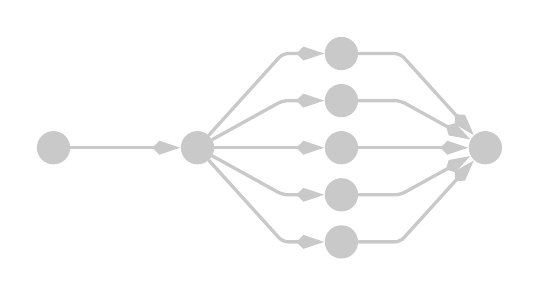
\begin{tikzpicture}[codeouthl]
  \matrix[matrix of nodes,nodes={circle,fill},above right,ampersand replacement=\&,column sep=4em,row sep=.5em] {
           \&        \& |(3a)|~ \&        \\
           \&        \& |(3b)|~ \&        \\
    |(1)|~ \& |(2)|~ \& |(3c)|~ \& |(4)|~ \\
           \&        \& |(3d)|~ \&        \\
           \&        \& |(3e)|~ \&        \\
  };
  % wellp: c\graph[edges={very thick,-Kite}]{(1) -> (2) -> {(3a),(3b),(3c),(3d),(3e)} -> (4)};
  \scope[every path/.append style={draw,very thick,-Kite,rounded corners=2pt,line cap=round}]
  \path(1) -- (2);  \path(2) -- (3c); \path(3c) -- (4);
  \foreach\a in {a,b,d,e} {
    \path (2) -- ([xshift=-1.5em]3\a.west) -- (3\a.west);
    \path (3\a.east) -- ++(1.5em,0) -- (4);
  }
  \endscope
\end{tikzpicture}}
\def\PostTitlepage{\begin{tikzpicture}[overlay,remember picture]
\node[above right=.5cm,xshift=1cm,scale=.875] at(current page.south west) {\copy\titleimg};
\end{tikzpicture}}

\addbibresource{./references.bib}

\makeatletter
\newcommand*\md{\@ifstar{\@md}{\@md{0}}}% with star we can set handout state
\def\@md#1#2{\only<#2|handout:#1>{\llap{\color{shadeA}\textbullet~}}}
\newcommand*\mb[2][0]{\only<#2|handout:#1>{\rlap{\smash{\raisebox{-.66\baselineskip}{\color{shadeA}\textbullet}}}}}
\newcommand*\mh[2][0]{\only<#2|handout:#1>{\color{shadeA}\textbullet}}
\newcommand*\mdl[2][0]{\only<#2|handout:#1>{\llap{\smash{\raisebox{-.5\baselineskip}{\tikz{\fill[shadeA,rounded corners=1pt] (0,-.65mm) rectangle ++(2.15\p@,\baselineskip+.65mm);}}~}}}}
\makeatother


\setcounter{tocdepth}{4}
\newsavebox\pinguA \newsavebox\pinguB \newsavebox\pinguC

\usepackage[link]{qrcode}
% TODO
\outroright{% \smash{\raisebox{1.33cm/2}{
% \qrcode[height=1.33cm]{https://github.com/EagleoutIce/Episode-Recursion}}}\begin{tikzpicture}[remember picture,overlay]
% \node[above left,btdl@color@white,scale=.475] at (current page.south east) {\href{https://github.com/EagleoutIce/Episode-Recursion}{Slides and \LaTeX-sources on GitHub!}};
% \end{tikzpicture}
}

\long\def\commy#1{\smash{\tiny\fboxsep=1pt\fcolorbox{pingu@purple}{pingu@purple!10!white}{\bfseries #1}}}
\long\def\flo#1{\commy{Flo:~#1}}
\long\def\felix#1{\commy{Felix:~#1}}

\usepackage{xspace}
\def\LogoParallel{parallel\xspace}%{para\textit{ll}\/el\xspace}
\makeatletter
\def\sol@minted@setup#1#2#3{\lstset{style=#1,language=#2,lineskip=4pt,#3,escapeinside={/*}{*/}}}
\solsetmintedstyle{plain}% number}

\def\HStrut{\vphantom{\{\}g}}
% we do not nest inside tikzmarknode as this is not possible
\def\Snode#1{\tikzmarknode{#1}\HStrut}
\def\bnode#1#2{\rnode{#1}{\sbasic{#2}}}%
\def\rnode#1#2{\Snode{#1}#2\Snode{#1@}}
\def\CodeFileMarker#1{{\color{gray}\sffamily\fontseries{l}\tiny\llap{\faFileCodeO~\thinspace}#1}}

\def\SetupLstHl{%
\lstcolorlet{highlight}{codeouthl}%
\sol@list@define@styles{%
 {highlight: \@declaredcolor{sol@colors@lst@highlight}\upshape},%
}}

\begin{document}
\section{Motivation}
% \SidebarCite{book:javase15-std}
\begin{frame}{Motivation}
% FELIX&FLO
\end{frame}
% \SidebarReset
\section{Running Example}
\begin{frame}{Example Run!}
% FELIX (pfusch von Flo, gson kram)
\end{frame}
\section{\texorpdfstring{\textsc{gnu}}{GNU} Para\textit{ll}\/el}
\subsection{History}
\begin{frame}{History}
   % FELIX
   % Single-file to work easily, perl because seems to be widespeared, problem: opverhead (--tag option+, https://www.gnu.org/software/parallel/parallel_design.pdf)
\end{frame}

\subsection{Usage in Bash}
\makeatletter % faulheit!
\begin{frame}[c]{Pipes}
\centering
% \begin{layout-imageonly}
\begin{tikzpicture}[,codeouthl,every path/.append style={line cap=round,rounded corners=2pt}]
   \onslide<2->{\node[circle,minimum size=1cm,fill] (@) at(0,0) {};}
   \onslide<3->{\draw[{Kite[scale=.8]}-,very thick](@.west) to[edge node={node[above,black] {\textsc{stdin}}}] ++(-2,0) coordinate (@i);}
   \onslide<4->{\draw[-{Kite[scale=.8]},very thick](@.east) to[edge node={node[above,black] {\textsc{stdout}}}] ++(2,0) coordinate (@O);}
   \onslide<5->{\draw[-{Kite[scale=.8]},very thick](@.north) |- ++(2,.5) node[pos=.75,above,black] {\textsc{stderr}};}
   \onslide<6->{\node[below,darkgray] (wc) at(@.south) {\sbfamily\bbash{wc -l}};}
   \only<7->{
   \scope[xshift=-6cm]
   \onslide<7->{\node[circle,minimum size=1cm,fill] (@) at(0,0) {};
   \draw[{Kite[scale=.8]}-,very thick](@.west) to[edge node={node[above,black] {\textsc{stdin}}}] ++(-2,0) coordinate (@I);
   \draw[-{Kite[scale=.8]},very thick](@.east) to[edge node={node[above,black] {\textsc{stdout}}}] ++(2,0)  coordinate (@o);
   \draw[-{Kite[scale=.8]},very thick](@.north) |- ++(2,.5) node[pos=.75,above,black] {\textsc{stderr}};}
   \onslide<8->{\node[below,darkgray] (cat) at(@.south) {\sbfamily\bbash{cat makefile}};}
   \endscope
   }
   \only<9->{
      \draw[-Kite,very thick,codeouthl!70!white] (@o) -- (@i) coordinate[pos=.5] (@@);
      \path (@@|-wc) node[darkgray,xshift=-1mm] {\sbfamily\T{|}};
   }
   \only<10->{
      \draw[decorate,decoration={brace,mirror,amplitude=2pt},thick,black,sharp corners] ([yshift=-1.25cm]@I) to[edge node={node[below=2pt] {Producer}}] ([yshift=-1.25cm]@o);
      \draw[decorate,decoration={brace,mirror,amplitude=2pt},thick,black,sharp corners] ([yshift=-1.25cm]@i) to[edge node={node[below=2pt] {Consumer}}] ([yshift=-1.25cm]@O);
   }
   % TODO: next slide, connect them with the pipe symbol
   % TODO: make programs black to read them better
\end{tikzpicture}
% \end{layout-imageonly}
% each program run in the command line has three data streams connected to it:
% \begin{tikzpicture}[overlay,remember picture]
% \scope[shift={(current page.south west)},shift={(\beamer@leftmargin,1cm)}]
% \endscope
% \end{tikzpicture}
\end{frame}

\begin{frame}[c]{Pipes\rhead{II}}
\centering
% \begin{layout-imageonly}
\begin{tikzpicture}[,codeouthl,every path/.append style={line cap=round,rounded corners=2pt}]
   \node[circle,minimum size=1cm,fill] (@) at(0,0) {};
   \draw[{Kite[scale=.8]}-,very thick](@.west) to[edge node={node[above,black] {\textsc{stdin}}}] ++(-2,0) coordinate (@i);
   \draw[-{Kite[scale=.8]},very thick](@.east) to[edge node={node[above,black] {\textsc{stdout}}}] ++(2,0) coordinate (@O);
   \draw[-{Kite[scale=.8]},very thick](@.north) |- ++(2,.5) node[pos=.75,above,black] {\textsc{stderr}};
   \onslide<4->{\node[below,darkgray] (wc) at(@.south) {\sbfamily\bbash{xargs gzip}};
      \foreach \a in {0,60,...,359} {
         \path ([yshift=-1mm]@)++(\a:2mm) node[btdl@color@background] {\huge\textbullet};
      }
   }% use --keep! and maybe --recursive for data

   \scope[xshift=-6cm]
   \node[circle,minimum size=1cm,fill] (@) at(0,0) {};
   \draw[{Kite[scale=.8]}-,very thick](@.west) to[edge node={node[above,black] {\textsc{stdin}}}] ++(-2,0) coordinate (@I);
   \draw[-{Kite[scale=.8]},very thick](@.east) to[edge node={node[above,black] {\textsc{stdout}}}] ++(2,0)  coordinate (@o);
   \draw[-{Kite[scale=.8]},very thick](@.north) |- ++(2,.5) node[pos=.75,above,black] {\textsc{stderr}};
   \onslide<2->{\node[below,darkgray] (ls) at(@.south) {\sbfamily\bbash{ls}};}
   \onslide<3->{\node[below=2mm,inner sep=1.5mm,fill=gray!10!white,rounded corners=2pt,text width=3cm,text=black,align=left,font=\ttfamily,scale=.85] at([xshift=1cm]ls.south) {%
      Dockerfile\\
      run-docker\\
      data\\
      makefile\\
      \ldots
   };}
   % ls hat Probleme, ist hier nur als einfaches Beispiel:
   % https://unix.stackexchange.com/questions/128985/why-not-parse-ls-and-what-to-do-instead
   \endscope
   \draw[-Kite,very thick,codeouthl!70!white] (@o) -- (@i) coordinate[pos=.5] (@@);
   \path (@@|-wc) node[darkgray,xshift=-1mm] {\sbfamily\T{|}};
   % TODO: benchmarks
\end{tikzpicture}
% \end{layout-imageonly}
% each program run in the command line has three data streams connected to it:
\end{frame}

\begin{frame}[c]{Pipes\rhead{III}}
   \centering
   % \begin{layout-imageonly}
   \begin{tikzpicture}[,codeouthl,every path/.append style={line cap=round,rounded corners=2pt}]
      \node[circle,minimum size=1cm,fill] (@) at(0,0) {};
      \draw[{Kite[scale=.8]}-,very thick](@.west) to[edge node={node[above,black] {\textsc{stdin}}}] ++(-2,0) coordinate (@i);
      \draw[-{Kite[scale=.8]},very thick](@.east) to[edge node={node[above,black] {\textsc{stdout}}}] ++(2,0) coordinate (@O);
      \draw[-{Kite[scale=.8]},very thick](@.north) |- ++(2,.5) node[pos=.75,above,black] {\textsc{stderr}};
      \onslide<4->{\node[below,darkgray] (wc) at(@.south) {\sbfamily\bbash{parallel gzip}};
         \foreach \a in {0,60,...,359} {
            \path ([yshift=-1mm]@)++(\a:2mm) node[btdl@color@background] {\huge\textbullet};
         }
      }% use --keep! and maybe --recursive for data

      \scope[xshift=-6cm]
      \node[circle,minimum size=1cm,fill] (@) at(0,0) {};
      \draw[{Kite[scale=.8]}-,very thick](@.west) to[edge node={node[above,black] {\textsc{stdin}}}] ++(-2,0) coordinate (@I);
      \draw[-{Kite[scale=.8]},very thick](@.east) to[edge node={node[above,black] {\textsc{stdout}}}] ++(2,0)  coordinate (@o);
      \draw[-{Kite[scale=.8]},very thick](@.north) |- ++(2,.5) node[pos=.75,above,black] {\textsc{stderr}};
      \onslide<2->{\node[below,darkgray] (ls) at(@.south) {\sbfamily\bbash{ls}};}
      \onslide<3->{\node[below=2mm,inner sep=1.5mm,fill=gray!10!white,rounded corners=2pt,text width=3cm,text=black,align=left,font=\ttfamily,scale=.85] at([xshift=1cm]ls.south) {%
         Dockerfile\\
         run-docker\\
         data\\
         makefile\\
         \ldots
      };}
      \endscope
      \draw[-Kite,very thick,codeouthl!70!white] (@o) -- (@i) coordinate[pos=.5] (@@);
      \path (@@|-wc) node[darkgray,xshift=-1mm] {\sbfamily\T{|}};
      % TODO: benchmarks
       TODO: parallel wirklich aufteilen
   \end{tikzpicture}
\end{frame}
% TODO: nice example clock:
% parallel -k echo {1}'{=3 $_=$_%2?":":" "=}'{2}{3} \
% ::: {0..12} ::: {0..5} ::: {0..9}
% from manual
% TODO: even with grouping, e.g by piping with 'sort' - a stateful operation which operates as "Flaschenhals"
% TODO: auch auf ::: und so eingehen % FLORIAN

% \subsection{The Running-Example}
\begin{frame}{Fun!}
   grafik und Code
% wann sinnvoll usw.
% bank beispiel mit java  %  FELIX
\end{frame}

\subsection{Distribution}
\begin{frame}{Distributed}
   grafik und Code
   % erweiterungen wei verteilt mehrere Systeme % FELIX (-ssh oder so)
\end{frame}
\subsection{Data Encoding}
\begin{frame}{Data Encoding}
      Code Json, vs. yaml, vs...
   % objekte % FLORIAN (gson und so)
\end{frame}
\subsection{Other Languages}
\begin{frame}[fragile]{Other Languages}
   Grafik und Code
\begin{uncoverenv}<2->
\begin{minted}{javascript}
const i = 32;
let m = i - 3;
\end{minted}
\end{uncoverenv}
   % verschiedene Sprache % FELIX
   % TODO: timeout option?
\end{frame}

\subsection{Recap} % maybe not as separate bot in the bottom?
\begin{frame}{Recap}
   \begin{itemize}[<+(1)->]
      \itemsep12pt
      \item Producer-Consumer
      \item stream-based communication \begin{itemize}
         \item cf. Javas functional streams
         \item serialization and deserialization % TODO: talk about advantages and disadvantages
         \item decoupled programs (e.g., no shared memory)
      \end{itemize}
      \item TODO: distribution @Felix (chapter F)
      \item lock-free etc because producer-consumer
      \item TODO: other stuff?
   \end{itemize}
\end{frame}

\section{Inner Workings}
% TOOD: siebar note for bash only https://devdocs.io/bash/pipelines | https://www.gnu.org/software/bash/manual/bash.pdf
\begin{frame}{About pipes}
\begin{itemize}
   \item Execute each program in own subshell
   \item TODO: not sequential: \url{https://stackoverflow.com/a/32946581} os we execute al steps in parallel for free (producer-consumer) \url{https://pubs.opengroup.org/onlinepubs/009695399/utilities/xcu_chap02.html\#tag_02_09_02}
   \item TODO: talk about redirection and sockets?
   \item load balacning \url{https://stackoverflow.com/questions/14039403/gnu-parallel-load-balancing}
   \item how does bash sync it?
\end{itemize}
% Semaphor => kann als solche verwendet werden
% Semaphor, Rechner Sockets, % FLO
% parallel nutzt die host-shell aus (deisgn: which shell to use, p11)
\end{frame}
\begin{frame}
 TODO: SPREADING BLOCKS OF DATA
 in \url{https://www.gnu.org/software/parallel/parallel.pdf}
 %  synchinc
\end{frame}

\section{Outlook?}
\begin{frame}{Look Out!}
% FELIX&FLO
% praktische Anwendungen
% optionen die wir nicht vorstellen
% gibt es eine geplante Weiterentwicklung? <- ne
% Alternativen: https://www.gnu.org/software/parallel/parallel_alternatives.pdf
% -pipe vs pipepart, disk buffering
% sql support --sql-master etc.
% table support
% shebang
\end{frame}

\end{document}